%=========================================================================
% (c) 2014, 2015 Josef Lusticky

\section{Egress traffic processing}\label{sec:linux-egress}
The previous sections described how the frame reception works and the processing path
when the routing subsystem decides to forward them.
After the routing decision is made and the {\it{skb}} is passed to the {\it{ip\_finish\_output()}} function,
it is further passed back to the link layer of the networking stack.
This part of the Linux networking also provides interface to the device drivers
and handles traffic control~\cite{understanding-internals}.

In reference to the egress traffic processing, there are two important functions in this part of the stack -
{\it{dev\_queue\_xmit()}} and {\it{dev\_hard\_start\_xmit()}}.
The {\it{ip\_finish\_output()}} function of the IPv4 stack passes the outgoing {\it{skb}}
to the {\it{dev\_queue\_xmit()}} function, which determines
whether the device is queueless of queueful.
If the device is queueless, such as Loopback or Virtual interface, then the {\it{skb}} is passed to
{\it{dev\_hard\_start\_xmit()}} directly without any traffic control mechanism involved.
The {\it{dev\_hard\_start\_xmit()}} function further prepares the {\it{skb}} for transmission
and passes it to the transmission function of the device driver,
which instructs the device to transmit the frame on the wire~\cite{understanding-internals}.

If the device is queueful, such as almost any hardware network adapter, {\it{dev\_queue\_xmit()}}
executes the traffic control first~\cite{understanding-internals}.
The traffic control implemented in the Linux kernel uses algorithms known as queuing disciplines
(often abbreviated as {\it{qdisc}})
to arrange the frames in the desired order for transmission~\cite{understanding-internals}.
Figure~\ref{fig:linux-egress-packet} shows a brief overview of this part of the stack.
\begin{figure}
	\centering
	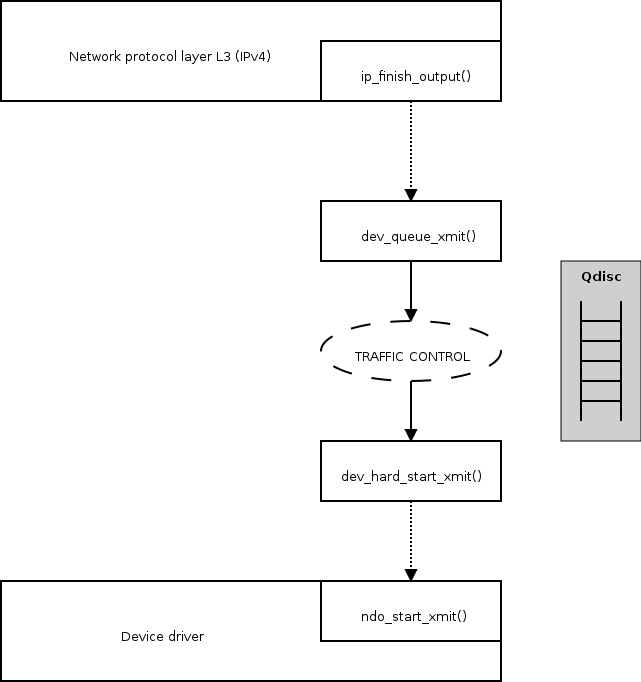
\includegraphics[width=10cm,keepaspectratio]{fig/kernel-layer2-flow.png}
	\caption{Egress packet processing}
	\label{fig:linux-egress-packet}
	\bigskip
\end{figure}

The Linux kernel supports various queuing disciplines, that can be configured by the {\it{tc}} utility.
The default queuing discipline for every network device is {\it{pfifo\_fast}}~\cite{linux-kernel-networking}.
The {\it{pfifo\_fast}} is a three-band First In First Out discipline.
As long as there are packets waiting in band 0, band 1 will not be processed.
Simliarly, packets from band 1 are always processed before packets from band 2.
Within each band, a simple FIFO rule apply.
The kernel inserts the packets to one of the band according to the Type of Service flag of the packet~\cite{tcpip-in-linux}.
A more detailed discussion of the traffic control and its queuing disciplines is outside the scope of this thesis.

After the packet has been selected for transmission by the traffic control, it is passed to the
{\it{ndo\_start\_xmit()}} function, which is implemented by the device driver.
The packet is inserted to the hardware transmit queue by the driver and transmitted.
The hardware transmit queue is implemented as a ring buffer (TX ring)
and the DMA controller of the device uses it to fetch the egress frames~\cite{kernel-source}.

The adpater uses interrupts to notify the kernel when the transmission fails or succeeds.
Simlarly to NET\_RX\_SOFTIRQ, which perfoms an interrupt-related work for incoming traffic,
the NET\_TX\_SOFTIRQ softirq handles the interrupt-related work for outgoing traffic.
The transmission code uses the softirq to mitigate interrupts in a similar fashion as the reception code.
Because different instances of the same softirq handler can run concurrently on different CPUs,
networking code is both low latency and scalable~\cite{understanding-internals}.

%=========================================================================
% (c) 2014, 2015 Josef Lusticky

\subsection{Transmit offloads}
Most of the adapters that support receive checksum offload
also support its counter-part transmission (Tx) checksum offload.
Tx checksum offload calculates TCP/UDP and
IP checksums of the packets in the hardware before they are transmitted on the wire.

A counter-part of LRO is TCP Segmentation Offload (TSO).
With a TSO-capable adapter, the kernel can prepare much larger packets for outgoing data
(e.g. up to 64KB in case of IPv4) and the adapter will re-segment the data into smaller packets according to the MTU~\cite{jls2009-gro}.
TSO is well supported in Linux -
for systems which are engaged mainly in sending of data,
it is sufficient to make 10~Gbps rate~\cite{jls2009-gro}.
TSO reduces the necessary CPU load, bus overhead, and cache impact to send a series of packets,
but it still does not require the adapter to actually know
anything about specific TCP connections -
the kernel still has to deal with the TCP states and ACKs~\cite{linux-and-tcp-offload-engines}.

The TCP Segmentation Offload is designed to work with TCP exclusively.
To mitigate this issue, the Generic Segmentation Offload (GSO) was implemented.
Performance improves even if the feature is emulated in the driver~\cite{jls2009-gro}.
Figure~\ref{fig:linux-tx-offloads} shows comparision of egress packet processing
with and without the above described offload mechanisms.
\begin{figure}
	\centering
	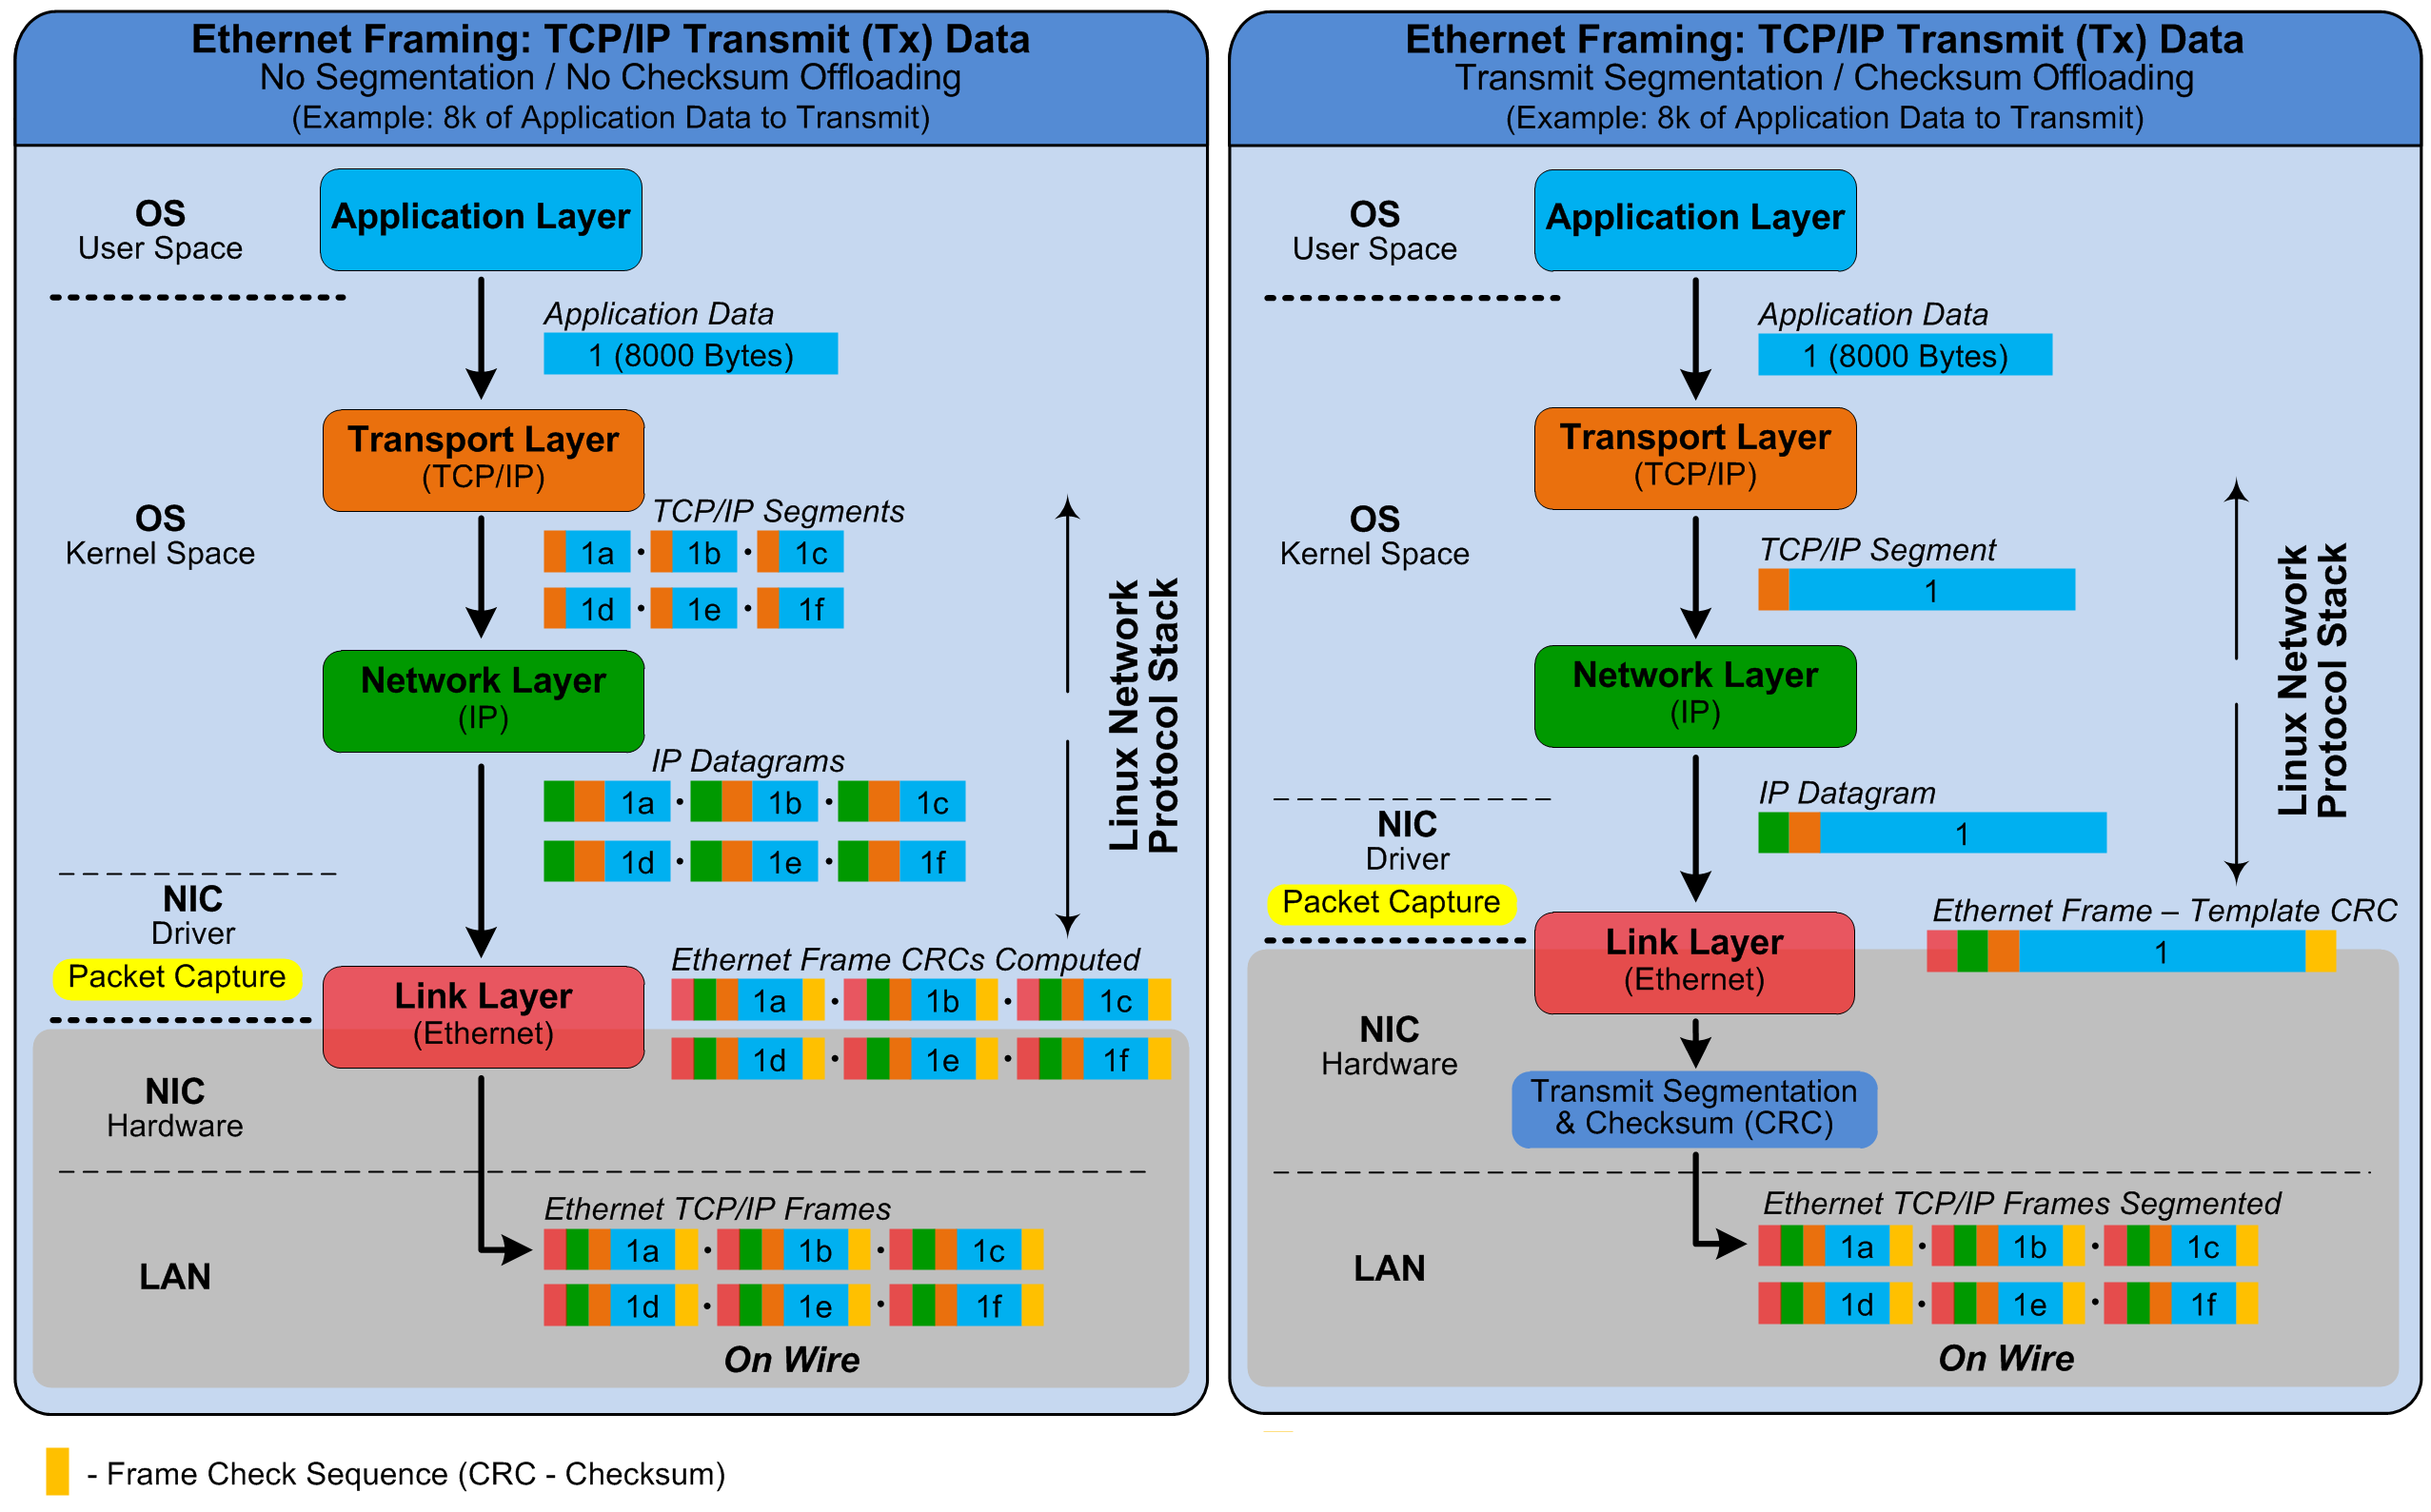
\includegraphics[width=15cm,keepaspectratio]{fig/tx-offloads.png}
	\caption{Transmit offloads (source:~\cite{nst-offloads})}
	\label{fig:linux-tx-offloads}
	\bigskip
\end{figure}

